
\section{Interesting Problems}
\subsection{Problem Description}


\begin{frame}[fragile]
  \frametitle{UVA 10937 -- Blackbeard the Pirate}

  {\smaller

    \begin{block}{}
      Blackbeard has to \structure{collect all treasures} (up to 10)
      in the island. He \alert{cannot cross} water or trees, and he
      must stay 1 square away from natives.

      \medskip

      Black beard speed is 1 square / second. How long does it take
      to get all treasure and return to the ship?
    \end{block}

\begin{verbatim}
10 10
~~~~~~~~~~       ~ -- Water, can't cross
~~!!!###~~       # -- Trees, can't cross
~##...###~       ! -- Treasure, get these!
~#....*##~       . -- Just sand
~#!..**~~~       * -- Natives, don't get close here.
~~....~~~~       @ -- Landing point, start and return here.
~~~....~~~
~~..~..@~~       The solution for this case is: 32
~#!.~~~~~~       How would YOU solve this problem?
~~~~~~~~~~
0 0
\end{verbatim}
}
\end{frame}

\begin{frame}
  \frametitle{UVA 10937 -- Blackbeard the Pirate}

  How would you solve this problem?\bigskip

  \begin{itemize}
    \item What is the data structure required for this problem?\bigskip

    \item What is the complexity of full search?\bigskip
    \begin{itemize}
      \item What are the solutions that you are searching?
      \item Max map size: $50\times50$, Max treasures: $10$
    \end{itemize}

    \item What is a more effective algorithm?
  \end{itemize}

\end{frame}

\subsection{Problem Solution -- Decomposition}
\begin{frame}[fragile]
  \frametitle{UVA 10937 -- Blackbeard the Pirate}

    \begin{block}{One way to solve this problem is to break it into two parts:}
      \begin{enumerate}
      \item Extract a weighted distance graph from the input map
      \item Solve the TSP for the graph
      \end{enumerate}
    \end{block}

    {\smaller
\begin{verbatim}
10 10
~~~~~~~~~~       ~ -- Water, can't cross
~~!!!###~~       # -- Trees, can't cross
~##...###~       ! -- Treasure, get these!
~#....*##~       . -- Just sand
~#!..**~~~       @ -- Landing point, return here.
~~....~~~~
~~~....~~~
~~..~..@~~
~#!.~~~~~~
~~~~~~~~~~
0 0
\end{verbatim}
  }
\end{frame}

\begin{frame}[fragile]
  \frametitle{UVA 10937 -- Blackbeard -- Extracting the graph}

  {\smaller
\begin{verbatim}
10 10
~~~~~~~~~~  ##########  # -- Obstacle (waters and trees)
~~!!!###~~  ##345#####  X -- Obstacles (natives, just for clarity)
~##...###~  ###..X####  . -- Path
~#....*##~  ##..XXX###  0-9 -- Nodes
~#!..**~~~  ##2.XXX###
~~....~~~~  ##..XX####
~~~....~~~  ###....###
~~..~..@~~  ##..#..0##
~#!.~~~~~~  ##1.######
~~~~~~~~~~  ##########
0 0
\end{verbatim}

\begin{itemize}
\item We can simply the graph into obstacles, paths and goals
\item We are only interested in the treasures and goals, so how to find the
  pairwise distance between treasures?
\item \alert{Answer}: \only<2>{BFS from each treasure/start point}
\item The result is a small graph with {\bf at most} 11 vertices.
\end{itemize}

  }
\end{frame}

\begin{frame}[fragile]
  \frametitle{UVA 10937 -- Blackbeard -- Extracting the graph}
  \begin{columns}
    \column{0.5\textwidth}

  {\smaller
\begin{verbatim}
##########
##345#####
###..X####
##..XXX###     BFS from each vertex
##2.XXX###     ------------------->
##..XX####     Not all paths shown
###....###
##..#..0##
##1.######
##########
\end{verbatim}}

    \column{0.5\textwidth}
  \begin{center}
    \begin{tikzpicture}[transform shape,label/.style={thin, draw=black, align=center,fill=white,font=\smaller},scale=1.1]
      \node[red vertex] (S) at (3,0) {0};
      \node[vertex] (ta) at (0,0) {1};
      \node[vertex] (tb) at (0,1.5) {2};
      \node[vertex] (tc) at (0,3) {3};
      \node[vertex] (td) at (1,3) {4};
      \node[vertex] (te) at (2,3) {5};
      \draw[edge] (S) -- node[label] {$8$} (ta);
      \draw[edge] (S) -- node[label] {$8$} (tb);
      \draw[edge] (S) -- node[label] {$10$} (td);
      \draw[edge] (td) -- node[label] {$1$} (tc);
      \draw[edge] (td) -- node[label] {$1$} (te);
      \draw[edge] (td) -- node[label] {$4$} (tb);
      \draw[edge] (tb) -- node[label] {$6$} (ta);
      \draw[edge] (S) -- node[label] {$11$} (te);
      \draw[edge] (tb) -- node[label] {$5$} (tc);
    \end{tikzpicture}
  \end{center}
  \end{columns}

  \begin{center}
    How do we find the minimal cycle starting in {\bf S}, passing by all vertices?
  \end{center}
\end{frame}

%% Explain TSP with DP and bit (Page 110)

\subsection{Traveling Salesman Problems}

\begin{frame}
  \frametitle{The Traveling Salesman Problem (TSP)}

  {\smaller
    \begin{block}{Problem Definition}
      You have $n$ cities, and their distances. Calculate the cost of
      the \structure{tour} that starts and ends at a city $s$, passing
      through all other cities.

      \medskip

      Exactly what we need! The path for all treasure!
  \end{block}
  \begin{center}
    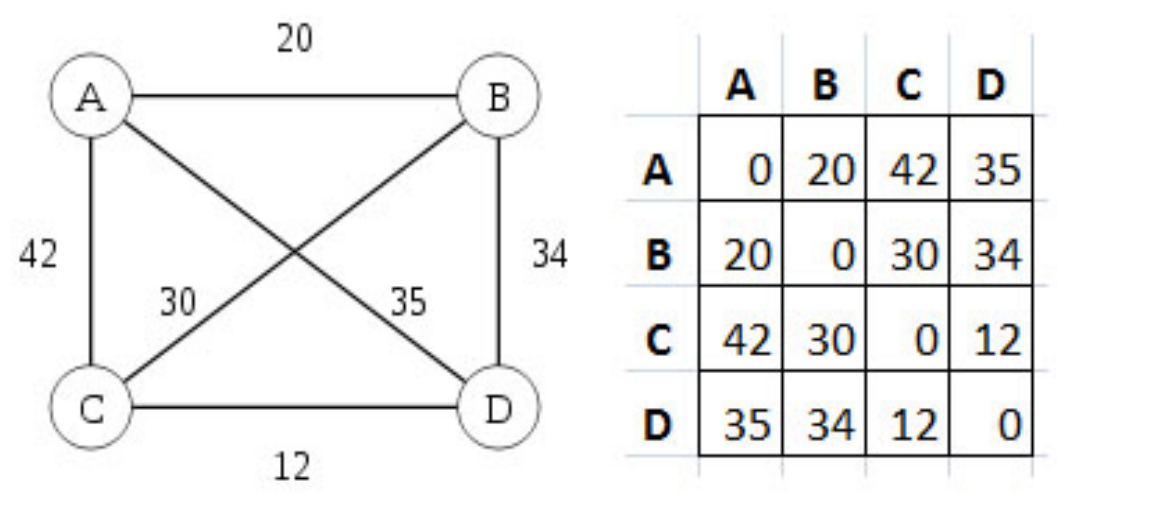
\includegraphics[width=0.5\textwidth]{../img/tsp_example}
  \end{center}

  In the graph above, we have $n=4$ cities and the minimal tour is
  A-B-C-D-A, with cost $20+30+12+35=97$.

  \medskip

  \alert{QUIZ:} What is the cost of solving TSP with complete search?
  }

  \hrulefill

  \hfill{\tiny Image from Steven Halim -- ``Competitive Programming''}

\end{frame}

\begin{frame}
  \frametitle{Characteristics of TSP}

  {\smaller
    \begin{block}{}
      \begin{itemize}
      \item A complete search for TSP costs $O(n!*n)$ -- \alert{Search
        each city permutation}.
      \item TSP is a {\bf NP-hard} problem. This means that there is
        no known polinomial algorithm to solve it.
      \item \alert{However!} For small values of $n$, there are some
        hacks to make the solution faster.
      \end{itemize}
    \end{block}

    \begin{exampleblock}{DP approach to TSP}
      The complete search for the TSP contains many \alert{repeated subsolutions}:
      \begin{itemize}
      \item S--A--B--C--$\ldots$--S
      \item S--B--A--C--$\ldots$--S
      \end{itemize}
      The minimum cost for C--$\ldots$--S is the same. Can we use
      \emph{memoization} to remember this cost?
    \end{exampleblock}
  }
\end{frame}

\begin{frame}
  \frametitle{DP approach to TSP (1) -- Idea}
    \begin{block}{}
      \begin{itemize}
      \item We have already visited the cities $S = \{s_1,s_2,\ldots,s_n\}, s_i \neq 0$
      \item We are {\bf now} in city $s_k \in S$
      \item What is the shortest path from $s_k$ to $0$, that passes in all cities $s_j \notin S$ ?
      \end{itemize}

      DP induction: shortest\_path($S$,$s_k$)
    \end{block}
    \begin{center}
      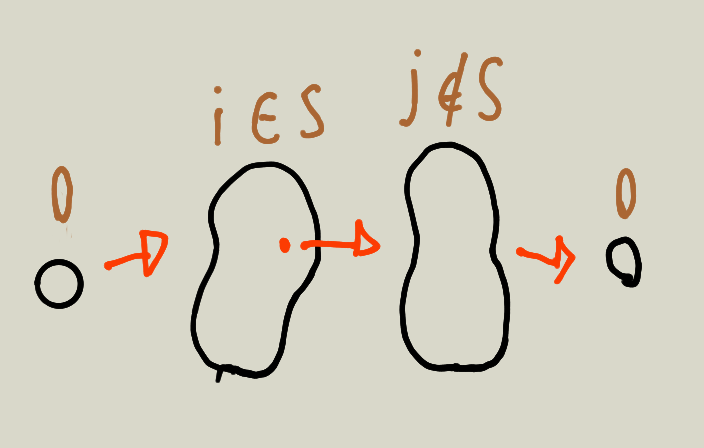
\includegraphics[width=0.4\textwidth]{img/DP_TSP}
    \end{center}
\end{frame}

\begin{frame}
  \frametitle{DP approach to TSP (2) -- DP Recurrence}

  {\smaller
    \begin{center}
      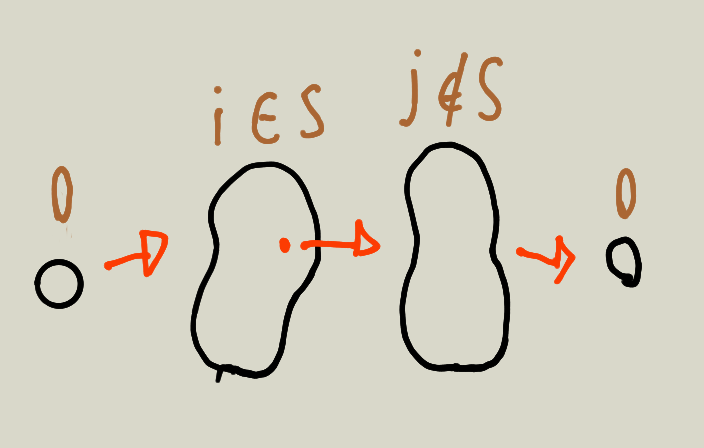
\includegraphics[width=0.35\textwidth]{img/DP_TSP}
    \end{center}
    \begin{block}{}
      \begin{itemize}
      \item We have visited all cities, and must return to the origin:\\
        shortest\_path($S_{\text{all}},s_k$) = $D(s_k,0)$
      \item We have visited some cites ($S$), and must find the next one:\\
        shortest\_path($S,s_k$) = $\text{min}_{s_i\notin S}
        (D(s_k,s_i) + \text{shortest\_path}(S\cup s_i,s_i))$
      \item Initial call:\\
        shortest\_path($S = \emptyset$,0)
      \end{itemize}
    \end{block}
  }
\end{frame}

\begin{frame}
  \frametitle{DP approach to TSP (3) -- Implementation}

    \begin{exampleblock}{}
      \begin{itemize}
      \item Our DP table is (\emph{all sets},\emph{all cities}) -- $2^n * n$
      \item We can represent a set of cities using a \structure{bitmask}
      \item At each call, we loop through all cities, so the complexity is $(O(2^n*n^2))$

        \bigskip

      \item TSP using full search: $O(n!*n)$
      \item TSP using DP: $O(2^n*n^2)$ -- Still low, but much better!
      \end{itemize}
    \end{exampleblock}
\end{frame}

\begin{frame}[fragile]
  \frametitle{DP approach to TSP (4) -- Sample Code}

{\smaller
  \begin{exampleblock}{}
\begin{verbatim}
int dp[n][1<<n] = -1
start = 0

visit(p,v):
   if (v == (1<<n) - 1):
      return cost[p][start]
   if dp[p][v] != -1
      return dp[p][v]

   tmp = MAXINT
   for i in n:
       if not(v && (1 << i):
           tmp = min(tmp,
                     cost[p][i] + visit(i, v | (1<<i)))

   dp[p][v] = tmp
   return tmp
\end{verbatim}
  \end{exampleblock}}
\end{frame}


\subsection{UVA 10003 -- Cutting Sticks}
\begin{frame}
  \frametitle{UVA 10003 -- Cutting Sticks}

  {\smaller
    \begin{block}{Problem Description}
      \begin{itemize}
      \item In a stick of length $l$ ($1 \leq l \leq 1000$)
      \item Make $N$ cuts at positions $\text{cuts} = \{c_1, c_2,
        \ldots, c_N\}$ $(1 \leq N \leq 50)$
      \item The cost of a cut is the size of the sub-stick that you cut.
      \item What order of cuts \structure{minimize the cost}?
      \end{itemize}
  \end{block}

  \medskip

  \structure{Example:} $l=100, N=3, \text{cuts}=\{25,50,75\}$

  \begin{center}
    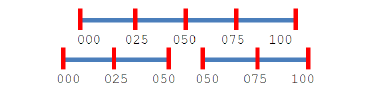
\includegraphics[width=0.6\textwidth]{../img/cuttingsticks}
  \end{center}

  \begin{itemize}
  \item Sequence 1: 25, 50, 75. Cost: 100 + 75 + 50 = 225
  \item Sequence 2: 50, 25, 75. Cost: 100 + 50 + 50 = 200
  \end{itemize}
  }
\end{frame}

\begin{frame}
  \frametitle{UVA 10003 -- Cutting Sticks -- Questions}

  {\smaller
    \begin{center}
      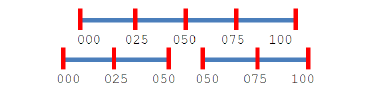
\includegraphics[width=0.55\textwidth]{../img/cuttingsticks}
      \begin{itemize}
      \item Sequence 1: 25, 50, 75. Cost: 100 + 75 + 50 = 225
      \item Sequence 2: 50, 25, 75. Cost: 100 + 50 + 50 = 200
      \end{itemize}
    \end{center}

    \begin{exampleblock}{Quiz 1}
      \begin{itemize}
      \item What is the algorithm for a full search?
      \item What is the complexity of this algorithm? And the maximum time?
      \end{itemize}
    \end{exampleblock}

    \begin{exampleblock}{Quiz 2}
      \begin{itemize}
      \item This problems smells of {\bf DP}...
      \item But what are the {\bf states}, and what is the {\bf transition}?
      \end{itemize}
    \end{exampleblock}

  }
\end{frame}

\begin{frame}
  \frametitle{UVA 10003 -- Cutting Sticks -- Recurrence}
  {\smaller
    \begin{center}
      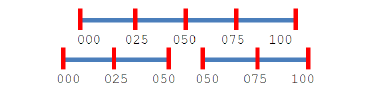
\includegraphics[width=0.6\textwidth]{../img/cuttingsticks}
      \begin{itemize}
      \item Sequence 1: 25, 50, 75. Cost: 100 + 75 + 50 = 225
      \item Sequence 2: 50, 25, 75. Cost: 100 + 50 + 50 = 200
      \end{itemize}
    \end{center}

    \begin{block}{Recurrence}
      Let's think of a \structure{Top-down DP} based on a recursive function:
      \begin{itemize}
      \item $A = \{0, c_1, c_2, \ldots c_N, N+2\}$ is the set of all cutting
        points, plus the start and end point.
      \item $\text{cost}(a_i,a_j) = \text{dist}(a_i,a_j) + \text{min}_{i\leq k\leq j}
        (\text{cost}(a_i,a_k) + \text{cost}(a_k,a_j))$
      \item $\text{cost}(a_i,a_i) = 0$
      \end{itemize}
      This requires at most a $(N,N)$ DP table for memoization, and O(N) for each iteration.
    \end{block}

  }
\end{frame}

\subsection{ACORN}
\begin{frame}
  \frametitle{UVA 1231 -- ACORN}

  \begin{columns}
    \column{0.4\textwidth}
    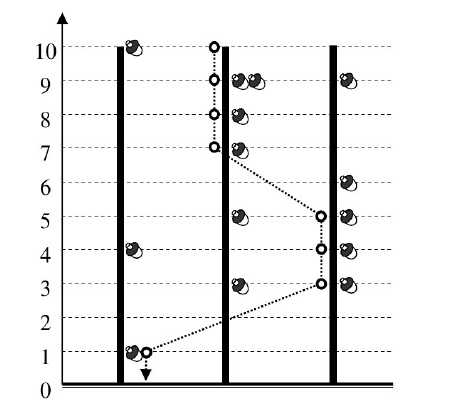
\includegraphics[width=1\textwidth]{img/acorn}
    \column{0.6\textwidth}

    \begin{itemize}
    \item Begin at the top of a tree, and get the maximum number of acorns.
    \item You can go down {\bf 1 height} on the tree.
    \item OR {\bf change tree} for the cost of {\bf f height}\\
      (In this figure, $f = 2$)

      \bigskip

    \item Number of trees: $ 1 \leq T \leq 2000$
    \item Height of trees: $ 1 \leq H \leq 2000$
    \item Length of fall : $ 1 \leq f \leq 500$
    \end{itemize}
  \end{columns}

  \begin{block}{}
    \begin{itemize}
      \item First, it is worth to think about the full search size;
      \item But this problem smells of DP -- can you think of a {\bf transition} and a {\bf state table}?
    \end{itemize}
  \end{block}
\end{frame}

\begin{frame}
  \frametitle{UVA 1231 -- ACORN -- Simple Recurrence}
  \begin{columns}[T]
    \column{0.3\textwidth}
    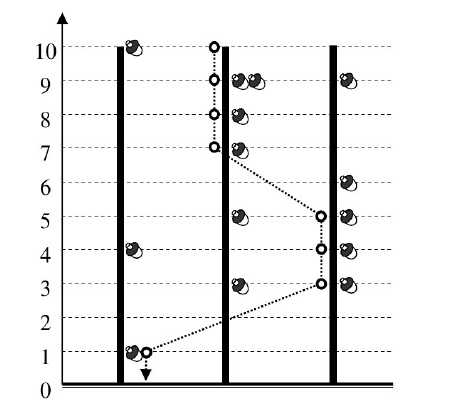
\includegraphics[width=1\textwidth]{img/acorn}
    \column{0.7\textwidth}
    \begin{block}{Simple Recurrence}
      \begin{itemize}
      \item acorn$[t_i][h]$ -- number of acorns in tree {\bf $t_i$} at height {\bf $h$}
        \bigskip

      \item cost$(t_i,0)$ = acorn$[t_i][0]$
        \bigskip

      \item cost$(t_i,j)$ = acorn$[t_i][j]$ + \\
        \hspace{1.6cm}max$_{k\neq t_i}($cost$(t_i,j-1)$, cost$(t_k,j-f))$\\
        (Don't forget to check $j-f < 0$)
        \bigskip

      \item Final cost: max$_{1\leq i \leq T}($cost$[t_i][H])$
      \end{itemize}
    \end{block}
  \end{columns}

  \vfill

  \begin{center}
    \alert{QUIZ:} What is the problem with this recurrence?
  \end{center}
\end{frame}

\begin{frame}
  \frametitle{UVA 1231 -- ACORN -- Better DP table}

    \begin{alertblock}{}
      The DP table of last slide is A[H][T], with size $2000*2000=4M$.
      Each function call is $O(H*T*T)$, so total complexity is
      $4M*2000=8B$
    \end{alertblock}

    \medskip

    \begin{itemize}
    \item Cost of changing tree is constant for any two trees.
    \item It is not necessary to keep all trees, only the best.
    \end{itemize}

    \medskip

    \begin{block}{Better Recurrence -- $O(H*T)$}
      We use the table dp$[H]$ which contains the best solution at height H.

      \medskip

      \begin{itemize}
      \item $\text{dp}[0] = \text{max}_{1\leq j\leq T}\text{acorn}[j][0]$
       \medskip

      \item $\text{acorn}[j][i] += \text{max}(\text{acorn}[j][i-1], \text{max}[i-f])$
        \medskip

      \item $\text{dp}[i] = \text{max}_{1\leq j\leq T}(\text{acorn}[j][i])$
      \end{itemize}
    \end{block}
\end{frame}

%\begin{frame}
%  \frametitle{UVA 1238 -- Free Parenthesis}
%\end{frame}

\section{Composite Problems}
\subsection{Fatman}
\begin{frame}
  \frametitle{UVA 295 -- Fatman!}
  \begin{center}
    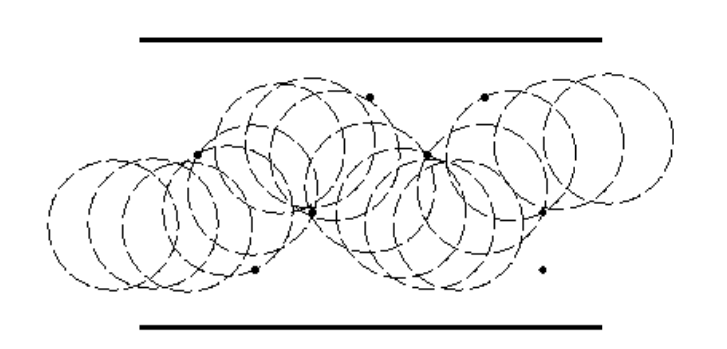
\includegraphics[width=0.5\textwidth]{img/fatman}
  \end{center}

  {\smaller
    \begin{block}{Problem Description}
      Find the {\bf maximum diameter D of the circle} that can pass the corridor.
      \begin{itemize}
      \item The corridor has length $L$ and width $W$;
      \item The corridor has $0 \leq N \leq 100$ obstacles, represented by $(x_i,y_i)$;
      \item Obstacles are {\bf points} with $0 \leq x_i \leq L, 0\leq y_i \leq W$;
      \end{itemize}
    \end{block}
  }
\end{frame}

\begin{frame}
  \frametitle{UVA 295 -- Fatman -- Breaking up the problem}
  \begin{center}
    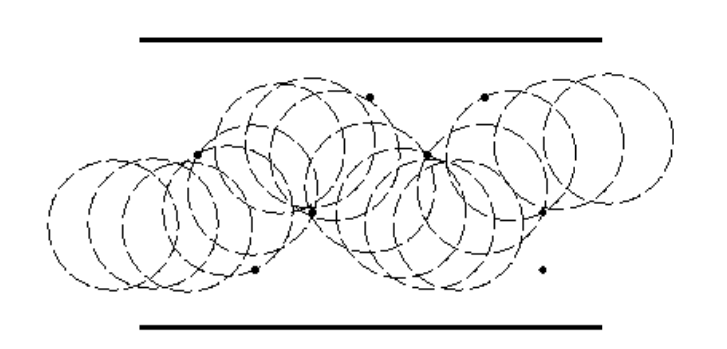
\includegraphics[width=0.5\textwidth]{img/fatman}
  \end{center}

  One way to solve some problems is to break them down into smaller
  components.

  \begin{block}{}
  \begin{enumerate}
  \item Is it possible for a circle of radius $R, 0 \leq R \leq W$ to pass?
  \item What is the maximum $R$ that can pass?
  \end{enumerate}
  \end{block}

  \alert{QUIZ}: Assume that (1) is ``fast enough'', how do we solve (2)?
\end{frame}

\begin{frame}
  \frametitle{UVA 295 -- Fatman -- Binary Search}

    \begin{block}{}
      \begin{itemize}
      \item Is it possible for a circle of size $0 \leq R \leq W$ to pass?
      \item What is the maximum $R$ that can pass?
      \end{itemize}
    \end{block}

    If we have a "fast" function $T(R)$ that tests if $R$ can pass or not, we can use {\bf Binary Search} to find the maximum $R$ that pass:

    \bigskip

    \begin{enumerate}
    \item Start with $R_l = 0, R_h = W$, Test $T(R_l+R_h /2)$;
    \item If fails, $R_h = R_l+R_h/2$, else $R_l = (R_l+R_h)/2$; repeat $T(R_l+R_h/2)$.
    \item Repeat until $R_h - R_l < 0.0001$.
    \end{enumerate}

    This requires log$_2(100*10000) = 20$ operations.

    \bigskip

    \alert{QUIZ:} How can we test $T(R)$ ``fast enough''?
\end{frame}

\begin{frame}
  \frametitle{UVA 295 -- Fatman -- Squeezing through}

    \begin{center}
      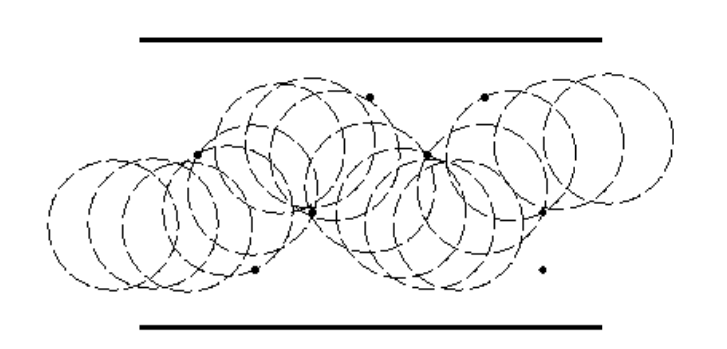
\includegraphics[width=0.4\textwidth]{img/fatman}
    \end{center}

    \begin{itemize}
    \item R can pass between two objects $i$ and $j$ if \emph{euclid}$(i,j) \geq R$
    \item R can pass between an object $i$ and a wall if $y_i \geq R || y_i \leq W-R$
    \end{itemize}

    \begin{exampleblock}{Algorithm for T(R)}
      \begin{itemize}
      \item Create a Graph $G$ where the obstacles and walls are vertices;
      \item If R can {\bf not} pass between $i$ and $j$, add an Edge $E_{ij}$;
      \item If there is a {\bf path} between both walls, \alert{R cannot pass};
      \end{itemize}
    \end{exampleblock}
\end{frame}

\begin{frame}[fragile]
  \frametitle{UVA 295 -- Fatman -- Squeezing through}

  {\smaller
  \begin{block}{T(R) sample code -- part 1, construct graph}
\begin{verbatim}
def test(R):
  nb = []                  # list of neighbor list
  for i in range(len(N)+2): nb[i] = list()

  for i in range(len(N)):  # N is list (x,y) of obstacles
    if (N[i][1] < R): nb[0].append(i+1)
    if (W - N[i][1] < R): nb[len(N)+1].append(i+1)
    if (i+1) in nb[0] and (i+1) in nb[len(N)+1]: return 0  # quick check 1
  if not (len(nb[0]) and len(nb[len(N)+1]): return 1       # quick check 2

  for i in range(len(N)):
    for j in range(len(N)):
      if dist(N[i],N[j]) < R: nb[i+1].append(j+1)
  ... next we test the graph ...
\end{verbatim}
  \end{block}
  }
\end{frame}


\begin{frame}[fragile]
  \frametitle{UVA 295 -- Fatman -- Squeezing through}


  {\smaller
    \alert{QUIZ:} What is the total cost of this approach?

    \begin{block}{T(R) sample code -- part 2, testing the graph}
\begin{verbatim}
def test(R):
  nb = []                  # list of neighbor list
  for i in range(len(N)+2): nb[i] = list()
  for i in range(len(N)):   ... border test ...
  for i in range(len(N)):
    for j in range(len(N)): ... build graph ...

  curnode = 0; visited = list(); tovisit = list()
  while 1: # DFS
    if (curnode == len(N)+1) return 0   # reached wall
    visited.add(curnode)
    for i in nb[curnode]: tovisit.append(i)
    while(curnode in visited):
       if not (len(tovisit)): return 1  # not reached wall
       curnode = tovisit.pop()
\end{verbatim}
    \end{block}
  }
\end{frame}

\subsection{Copying Books}
\begin{frame}[fragile]
  \frametitle{UVA 714 -- Copying books}

  {\smaller
    \begin{block}{Problem Description}
      \begin{itemize}
      \item There are $M$ books and $K$ scribes $(1 \leq K \leq M \leq 500)$.
      \item The each book has $p_i$ pages $(1 \leq p_i \leq 1000000)$
      \item Assign books to each scribe, and {\bf minimize} maximum job.
      \item Books must be assigned in blocks.
      \end{itemize}
    \end{block}

\begin{verbatim}
9 3
Input 1: 100 200 300 400 500 600 700 800 900
Output 1: 100 200 300 400 500 / 600 700 / 800 900 (max 1700)

5 4
Input 2: 100 100 100 100 100
Output 2: 100 / 100 / 100 / 100 100 (max 200)
\end{verbatim}

\begin{itemize}
\item \alert{QUIZ:} Describe the full search (and complexity)
\item \alert{QUIZ:} Describe a better algorithm?
\end{itemize}

  }
\end{frame}

\begin{frame}[fragile]
  \frametitle{UVA 714 -- Copying books -- Decomposition approach}

\begin{verbatim}
9 3
Input 1: 100 200 300 400 500 600 700 800 900
Output 1: 100 200 300 400 500 / 600 700 / 800 900 (max 1700)

5 4
Input 2: 100 100 100 100 100
Output 2: 100 / 100 / 100 / 100 100 (max 200)
\end{verbatim}

\vfill

    \begin{itemize}
    \item Someone has probably suggested DP. It is certainly possible.
    \item We could also use ``Binary Search + Test'' from the last problem:
      \begin{itemize}
      \item Binary search the maximum cost (100000*500 = 26 comparisons)
      \item Test if the maximum cost is possible (T(max))
      \item \alert{QUIZ:} What is a ``fast enough'' algorithm for T(max)?
      \end{itemize}
    \end{itemize}
\end{frame}

\begin{frame}[fragile]
  \frametitle{UVA 714 -- Copying books -- Testing a solution}
  {\smaller

\begin{verbatim}
9 3
Input 1: 100 200 300 400 500 600 700 800 900
Output 1: 100 200 300 400 500 / 600 700 / 800 900 (max 1700)
\end{verbatim}

\vfill

\begin{block}{One possible Test: Greedy Algorithm to test Maximum M}
\begin{verbatim}
def test(M):
  scribe = 0; book = 0;
  while scribe < K:
    sum = 0
    while sum + page[book] < M:
      sum += page[book]; book += 1
      if book == M: return 1   # assigned all books
    scribe ++
  return 0                     # did not assign all books
\end{verbatim}
\end{block}

\begin{alertblock}{}
  Caution: This code gives WA -- in case of tie, you need lowest jobs first!
\end{alertblock}
  }
\end{frame}

%\subsection{How Big is it?}
%\begin{frame}
%  \frametitle{UVA 10012 -- How big is it?}
%\end{frame}

\section{The Last Problem!}

\subsection{Messages}
\begin{frame}
  \frametitle{Take-home messages}
    \begin{block}{Composite Problems}
      Many interesting problems use a combination of algorithms:
      \begin{itemize}
      \item Blackbeard: BFS + TSP
      \item Fatman: Geometry + Graph + Binary Search
      \item Books: Greedy + Binary Search
      \end{itemize}
    \end{block}

    \vfill

    \begin{alertblock}{Do not forget simple approaches}
      Binary-search-and-test is {\bf very powerful} if:
      \begin{itemize}
      \item You need to find a bounded maximum or minimum;
      \item The feasibility test is simple to perform; (code-simple)
      \end{itemize}
  \end{alertblock}
\end{frame}

\subsection{A careful Approach}
\begin{frame}[fragile]
  \frametitle{UVA 1079 -- A careful Approach}

  {\smaller
    \begin{block}{Problem Description}
      \begin{itemize}
      \item Choose the landing time $t_i$ for $2 \leq N \leq 8$ planes;
      \item The minimum gap $|t_i - t_j|$ must be as large as possible;
      \item Each plane $i$ has a maximum and minimum allowed landing time:\\
        $0 \leq \text{min}_i \leq t_i \leq \text{max}_i \leq 1440$
      \end{itemize}
    \end{block}

\begin{verbatim}
Input:               Solution:
3 planes             Maximum Minimum Gap: 7.5 minutes
1- 0 to 10           P1 - Arrive at 0
2- 5 to 15           P2 - Arrive at 7.5
3- 10 to 15          P3 - Arrive at 15
\end{verbatim}
  }

  \alert{Final Quiz:} Let's solve this problem\\
  (hint: it is composite of 3 problems!)
\end{frame}
